\newpage
\section{Definizione del Prodotto}

\subsection{Metodo e formalismo di specifica}
Verrà qui esposta l'architettura di Premi ad alto livello seguendo un approccio top-down$_G$: verranno prima descritti i package$_G$ e le loro dipendenze e successivamente le singole classi contenute al loro interno. I diagrammi delle classi e dei package$_G$ seguono il formalismo UML$_G$2.0 e la struttura dei package segue una prassi ("best practice$_G$") di AngularJS$_G$ che propone una suddivisione dei componenti per funzionalità dell'applicazione in alternativa alla classica suddivisione Model-View-Controller$_G$, la quale potrebbe collassare nel caso di implementazione di funzionalità aggiunte all'applicazione. Ad esempio se si hanno più di 10 controllers, views e directories potrebbe essere necessario effettuare una lunga ricerca nell'albero delle directories per trovare il file desiderato, rendendo quindi tale approccio più difficile da mantenere per applicazioni di medie o grandi dimensioni. Al contrario, una struttura modulare, permette una migliore gestione dei file per quanto riguarda applicazioni medio-grandi.
Si illustreranno poi i Design Pattern utilizzati nella fase di progettazione ad alto livello e si descriveranno le interazioni dell'utente con l'applicazione attraverso i diagrammi di attività$_G$.


\subsection{Presentazione dell'architettura generale del sistema}

I componenti sono stati suddivisi prima in base al loro contributo a specifiche funzionalità del software e solo successivamente per appartenenza ai ruoli del pattern MVC$_G$. Questo aumenta la chiarezza espositiva dei diagrammi, evita la creazione di package$_G$ contenenti un numero eccessivo di classi e aiuta a compiere verifiche mirate a singoli componenti. \\
È importante specificare che il framework AngularJS$_G$ unisce view e controller attraverso una dichiarazione esterna a entrambi, che fa parte del meccanismo detto di \textit{routing} o di reindirizzamento dell'utente; view e controller inoltre non sanno di essere collegati tra loro e comunicano attraverso un oggetto chiamato \textit{\$scope}. Questo rende l'architettura sia di tipo Model-View-Controller$_G$ che di tipo Model-View-ViewModel$_G$. \\
Per motivi di leggibilità \$scope e routing non verranno rappresentati in modo esplicito nei diagrammi dei package e delle classi di questo documento, ma sono comunque da considerarsi impliciti nelle dipendenze tra i view e controller dei componenti. \\
\subsection{Server}

\begin{figure}[h]
\begin{center}
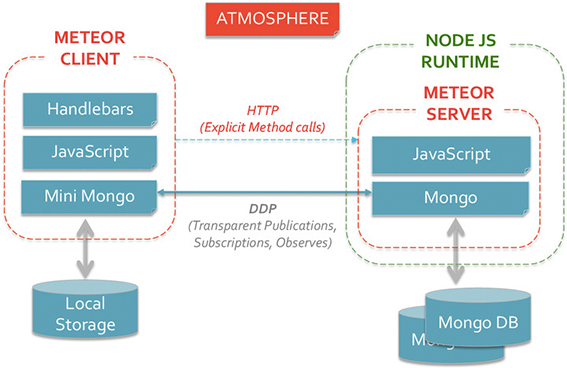
\includegraphics[scale=0.35]{img/meteor_architettura.jpg}
\caption{Schema archittetura}
\end{center}
\end{figure}

La comunicazione con la componente server avviene tramite la libreria Node.js$_G$ già implementata in MeteorJS$_G$. Con questa componente l'archittetura permette di realizzare un'applicazione asincrona, che a differenza del modello classico client-server permette di eseguire operazioni utili durante l'attesa di ricevere o di modificare un dato richiesto.
Nel server sono presenti delle funzioni che permettono al client di reperire i dati dal database MongoDB$_G$ residente nel server. In locale vengono scaricati solo i file richiesti che servono in quel momento. Ogni modifica ai dati viene effettuata prima nel database locale Minimongo$_G$; solo successivamente MeteorJS esegue in automatico in background la sincronizzazione tra Minimongo$_G$ e MongoDB$_G$.
\clearpage
\newpage
\section{Diagramma dei Package}
Di seguito vengono rappresentati i componenti principali del sistema e le loro dipendenze. \\
Package contenenti parti del prodotto relative alla componente \textit{Model} sono stati colorati di rosso; quelli relativi alla componente \textit{Controller} o \textit{ViewModel} sono stati colorati di verde, mentre quelli che racchiudono i template delle \textit{View} sono stati colorati di arancio. Questa scelta ha il solo scopo di facilitare la comprensione della struttura del sistema e non si basa su alcun standard UML$_G$.

\begin{figure}[h]
\begin{center}
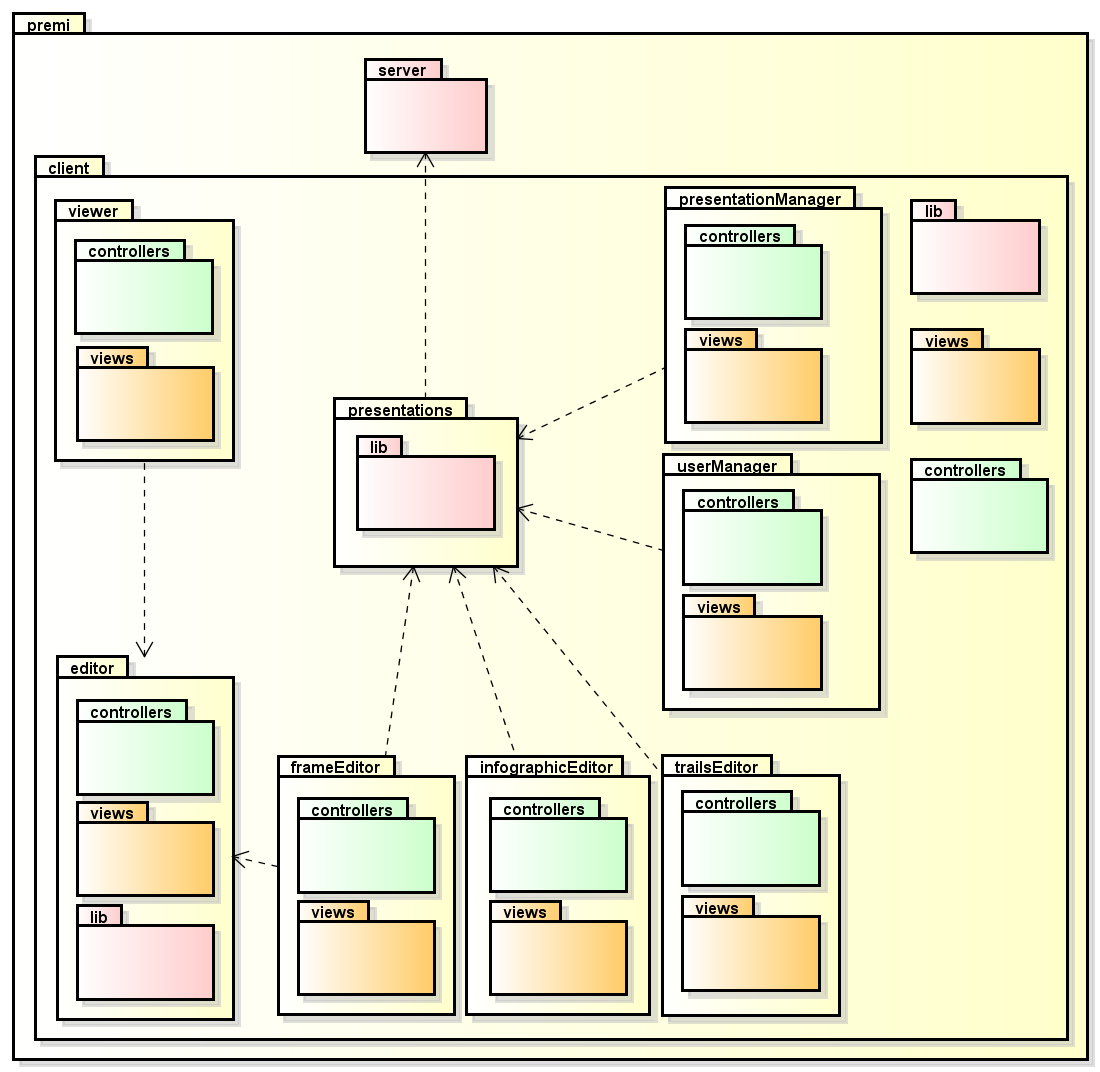
\includegraphics[scale=0.40]{img/diapkg/package.png}
\caption{Diagramma dei package di Premi.}
\end{center}
\end{figure}

L'applicazione è costituita da un solo package$_G$ principale chiamato \code{premi}; al suo interno sono presenti:
\begin{itemize}
\item \code{premi.server} contiene una libreria di metodi per l'inserimento, l'aggiornamento e la rimozione dei dati presenti nel database$_G$;
\item \code{premi.client} è il package principale che gestisce le funzionalità offerte all'utente. Contiene al suo interno tutti i package relativi al lato client dell'applicazione, tra cui anche il template$_G$ ed il controller$_G$ della vista principale, e le librerie esterne adottate per la realizzazione di alcune parti dell'applicazione;
\item \code{premi.client.header} contiene i files necessari alla creazione e alla visualizzazione dell'header$_G$ dell'applicazione;
\item \code{premi.client.presentation} contiene un'interfaccia per l'utilizzo dei metodi di inserimento, aggiornamento e rimozione dei dati presenti nel server; contiene anche delle classi per la gestione delle presentazioni dell'utente;
\item \code{premi.client.presentationManager} consente all'utente di creare, modificare o eliminare le  presentazioni;
\item \code{premi.client.editor} è lo scheletro dell'editor delle presentazioni. Al suo interno sono presenti le classi che modellano gli elementi che compongono la presentazione;
\item \code{premi.client.frameEditor} è la parte di editor che si occupa di creare, modificare o cancellare i Frame$_G$ contenuti nella presentazione;
\item \code{premi.client.infographicEditor} è a parte di editor che permette il posizionamento dei Frame$_G$ o di altri elementi all'interno di un poster;
\item \code{premi.client.trailsEditor} è la parte di editor che permette all'utente di ordinare i Frame per la creazione di uno o più percorsi di presentazione;
\item \code{premi.client.userManager} è il package$_G$ di gestione dei dati dell'utente; fornisce le procedure per la registrazione, il login, il cambio di password, ecc;
\item \code{premi.client.viewer} racchiude gli elementi necessari alla visualizzazione della presentazione nei vari contesti previsti(presentazione live, pubblica e privata).
\end{itemize}

\clearpage